\begin{figure}
\begin{tabular}{cc}
\begin{subfigure}[b]{0.55\textwidth}
\begin{center}
{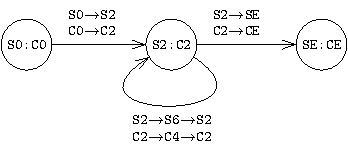
\includegraphics[scale=0.87]{figStrlenArrProductCfg.pdf}}
\end{center}
\caption{\label{fig:llproduct}Product CFG for Array-based Implementation}
\end{subfigure}%
&
\begin{subfigure}[b]{0.45\textwidth}
\begin{center}
\begin{footnotesize}
\begin{tabular}{|c|l|}
\hline
\tt PC-Pair & \multicolumn{1}{c|} {\tt Invariants} \\
\hline
\hline
\Tstrut ${\tt (S0:C0)}$ &
${\tt {\circled{P}}\  s_{S}\indEq{}Cstr^{char[]}_{m}(s_{C})}$ \\
\Tstrut \BBstrut \multirow{2}{*}{${\tt (S2:C2)}$} &
${\tt {\scriptsize \circled{I1}}\  s_{S}\indEq{}Cstr^{char[]}_{m}(s_{C})}$ \\ & ${\tt {\scriptsize \circled{I2}}\  len_{S}=i_{C}}$ \\
\Tstrut \BBstrut ${\tt (SE:CE)}$ &
${\tt {\circled{E}}\  ret_{S}=ret_{C}}$ \\
\hline
\end{tabular}
\end{footnotesize}
\end{center}
\caption{\label{fig:XX}Invariants Table for Array-based Implementation}
\end{subfigure}%
\\
\begin{subfigure}[b]{0.55\textwidth}
\begin{center}
{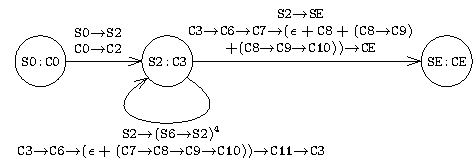
\includegraphics[scale=0.87]{figStrlenClProductCfg.pdf}}
\end{center}
\caption{\label{fig:llproduct}Product CFG for Chunked linked list-based Implementation}
\end{subfigure}%
&
\begin{subfigure}[b]{0.45\textwidth}
\begin{center}
\begin{footnotesize}
\begin{tabular}{|c|l|}
\hline
\tt PC-Pair & \multicolumn{1}{c|} {\tt Invariants} \\
\hline
\hline
\Tstrut ${\tt (S0:C0)}$ &
${\tt {\circled{P}}\  s_{S}\indEq{}Cstr^{clnode}_{m}(cl_{C}, 0)}$ \\
\Tstrut \BBstrut \multirow{2}{*}{${\tt (S2:C4)}$} &
${\tt {\scriptsize \circled{I1}}\  s_{S}\indEq{}Cstr^{clnode}_{m}(cl_{C}, 0)}$ \\ & ${\tt {\scriptsize \circled{I2}}\  len_{S}=i_{C}}$ \\
\Tstrut \BBstrut ${\tt (SE:CE)}$ &
${\tt {\circled{E}}\  ret_{S}=ret_{C}}$ \\
\hline
\end{tabular}
\end{footnotesize}
\end{center}
\caption{\label{fig:XX}Invariants Table for Chunked linked list-based Implementation}
\end{subfigure}%
\end{tabular}
\vspace{-10px}
\caption{\label{fig:strlenall}Product CFGs and Invariants Tables for two Implementations of Strlen Spec}
\vspace{-8px}
\end{figure}